\section{Digitaltechnik 1}
\subsection{Wahrheitstabelle, KDNF, KKNF, Y-Diagramm}
\begin{tabular}{ll}
  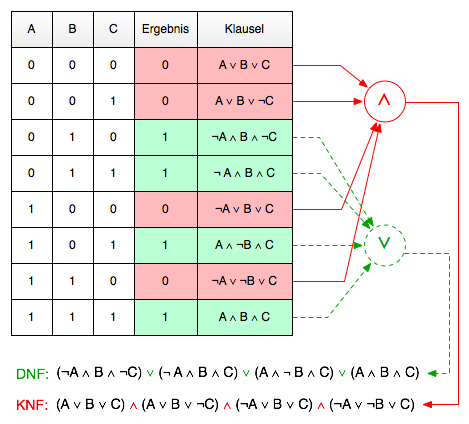
\includegraphics[width=0.4\textwidth]{pics/KNFDNF} &
  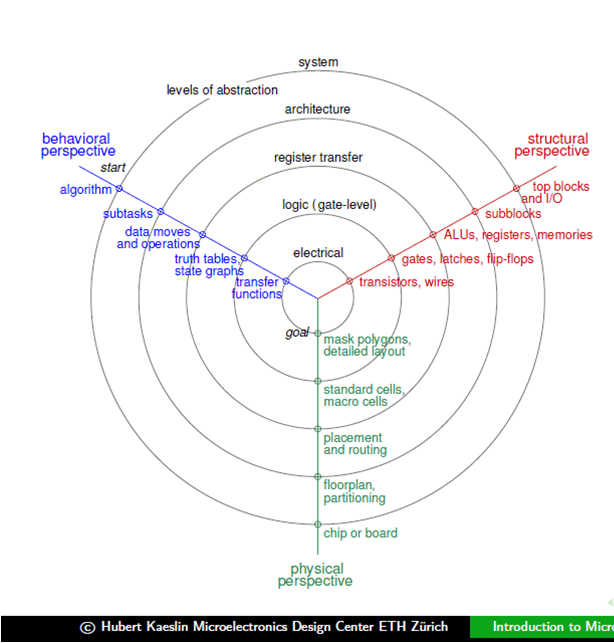
\includegraphics[width=0.3\textwidth]{pics/ydiagramm}
\end{tabular}
\\
Kurzschreibweisen:\\
KNF: $ a = \&([1],[2],3) $ \\
DNF: $ b = \#([1],[3],37) $ \\
Zeugs in eckigen Klammern bedeutet don't care.
\subsection{Karnaugh-Diagramm}
\begin{tabular}{lll}
  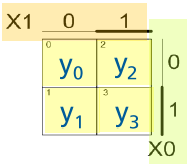
\includegraphics[width=0.1\textwidth]{pics/kv/2erKV} & 
  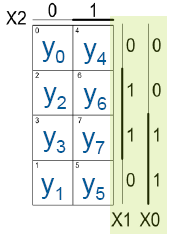
\includegraphics[width=0.1\textwidth]{pics/kv/3erKV} &
  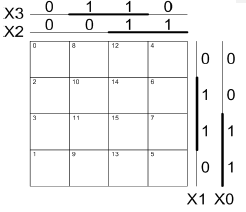
\includegraphics[width=0.2\textwidth]{pics/kv/4erKV}\\
\end{tabular}
\subsection{Arbeiten mit KV-Diagramm}
\begin{enumerate}
\setlength{\itemsep}{1pt}
  \setlength{\parskip}{0pt}
  \setlength{\parsep}{0pt}
\item Aufstellen der Wahrheitstabelle.\\
\item "Ubertragen der Werte der Wahrheitstabelle in KV Diagramm.\\
\item M"oglichst grosse Gruppen a $2^n$ Felder bilden.\\
\item
\begin{tabular}{ll}
  DNF & KNF \\
  Gruppen von Feldern mit Wert 1 oder d & Gruppen von Feldern mit Wert 0 oder d\\
  Primimplikanten: AND Verkn. & Primimplikanten: OR Verkn.\\
  OR Verkn. aller Primimpl. & AND Verkn. aller Primimpl.\\
\end{tabular}
\end{enumerate}

\begin{sidewaystable} 
\begin{tabular}{|c|c|c|c|c|c|c|c|c|}
\hline
Funktion & Buffer & NOT & AND & NAND & OR & NOR & EXOR & XNOR\\
& & Nicht & Und & Nicht Und & Oder & Nicht Oder & Exklusiv Oder & Nicht Ex. Oder\\
& & Inverter & Konjunktion & & Disjunktion & & Antivalenz & "Aquivalenz \\
\hline
Formel & a & $ \overline a $ & $ a \cdot b $ & $ \overline{a \cdot b} $ & $ a + b $ & $ \overline{a + b} $ & $ a \oplus b $ & $ \overline{a \oplus b} $\\
& a & $ \overline a $ & $ a \wedge b $ & $ \overline{a \wedge b} $ & $ a \vee b $ & $ \overline{a \vee b} $ & $ a \not= b $ & $ \overline{a \not= b} $ \\
& a & !a & $ a \& b $ & $ !(a \& b) $ & a\#b & !(a\#b) & a\$b & !(a\$b) \\
& & & & & & & $ a \veebar b $ & $ \overline{a \veebar b} $\\
\hline
& & & & & & & &\\
& 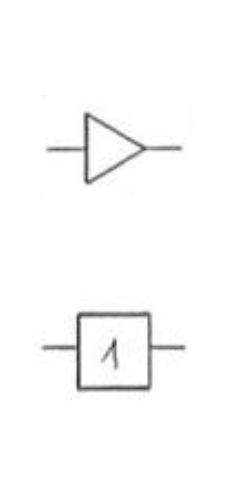
\includegraphics[width=0.08\textwidth]{pics/gates_symbol/buffer} & 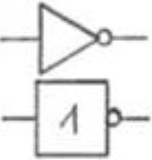
\includegraphics[width=0.08\textwidth]{pics/gates_symbol/not} & 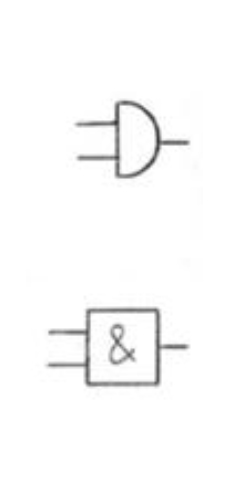
\includegraphics[width=0.08\textwidth]{pics/gates_symbol/and} & 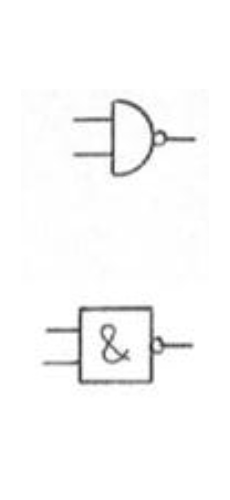
\includegraphics[width=0.08\textwidth]{pics/gates_symbol/nand} & 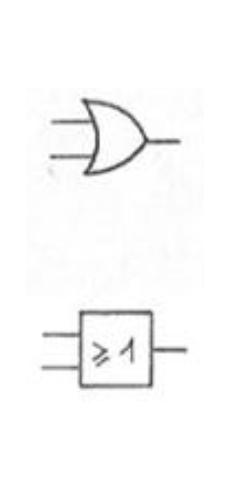
\includegraphics[width=0.08\textwidth]{pics/gates_symbol/or} & 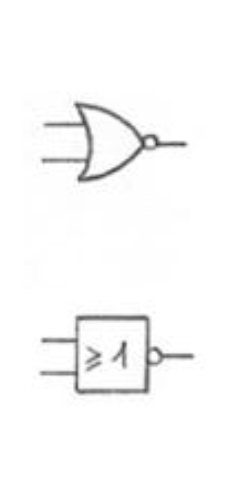
\includegraphics[width=0.08\textwidth]{pics/gates_symbol/nor} & 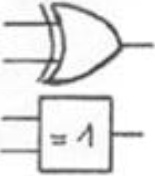
\includegraphics[width=0.08\textwidth]{pics/gates_symbol/exor} & 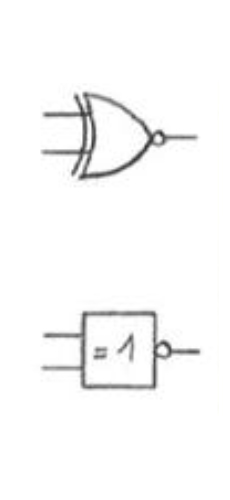
\includegraphics[width=0.08\textwidth]{pics/gates_symbol/xnor} \\
\hline
(0,0) & 0 & 1 & 0 & 1 & 0 & 1 & 0 & 1\\
(0,1) &   &   & 0 & 1 & 1 & 0 & 1 & 0\\
(1,0) & 1 & 0 & 0 & 1 & 1 & 0 & 1 & 0\\
(1,1) &   &   & 1 & 0 & 1 & 0 & 0 & 1\\
\hline
KDNF & \#(1) & \#(0) & \#(3) & \#(0,1,2) & \#(1,2,3) & \#(0) & \#(1,2) & \#(0,3) \\
KKNF & \&(0) & \&(1) & \&(0,1,2) & \&(3) & \&(0) & \&(1,2,3) & \&(0,3) & \&(1,2)\\
\hline
& & & & & & & &\\
& & 
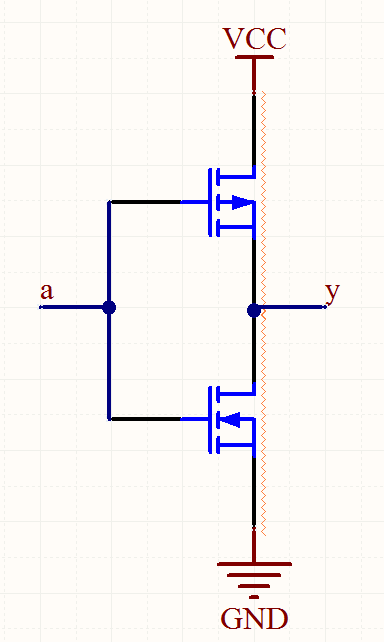
\includegraphics[width=0.12\textwidth]{pics/gates_schematic/inverter} &
$ \overline{NAND} $ &
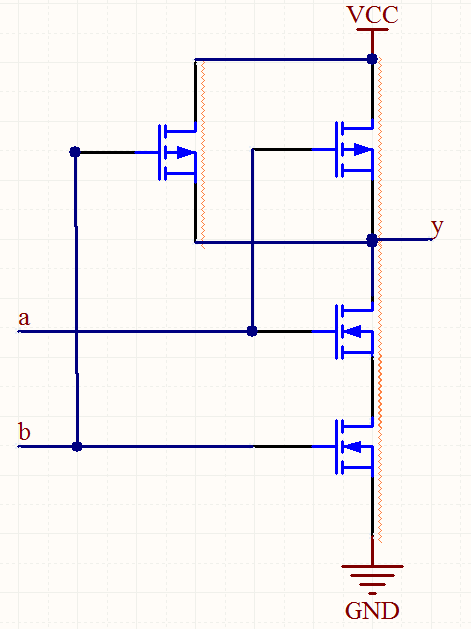
\includegraphics[width=0.12\textwidth]{pics/gates_schematic/NAND} &
$ \overline{NOR} $ &
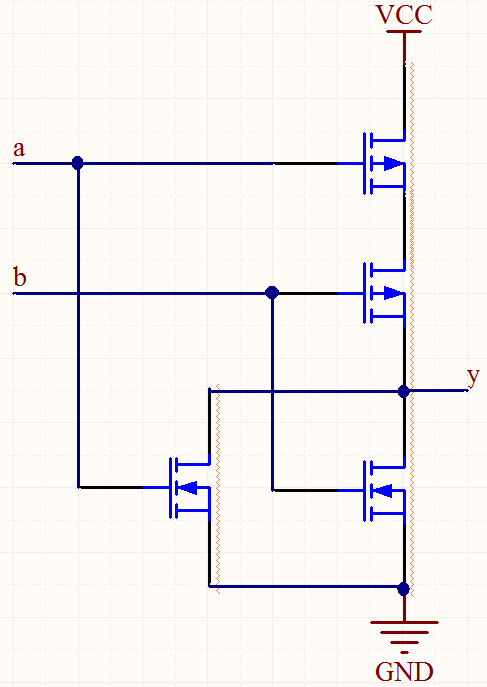
\includegraphics[width=0.12\textwidth]{pics/gates_schematic/NOR} &
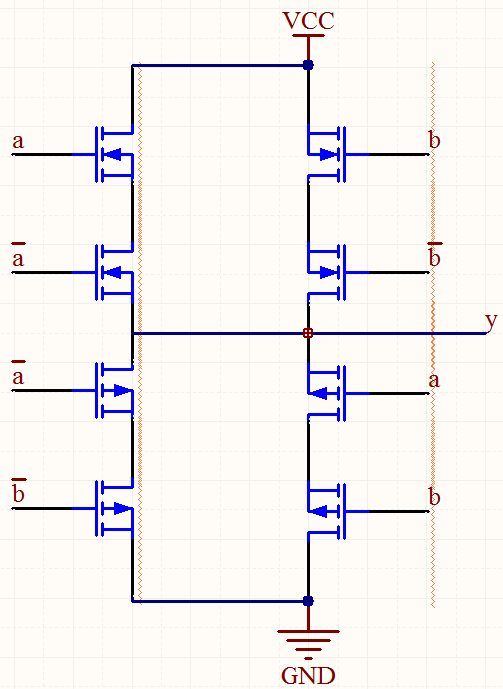
\includegraphics[width=0.12\textwidth]{pics/gates_schematic/XOR} &
\\
\hline
\#Trans & & 2 & 6 & 4 & 6 & 4 & 8 & \\
\hline
\end{tabular}
\end{sidewaystable}